\documentclass{standalone}
\usepackage{standalone}

\begin{document}

\subsection{Neural Network Design}
A three-layers feed forward supervised network is designed to suit the purpose. The input layers has 27 neurons, taking the 27 extracted features from the previous step. We used 40 neurons in output layer, because it has 40 different output as shown in \ref{table:OutputTypes}. In the hidden layer we have 180 neurons connecting input and output layers (including bias). Figure \ref{fig:PerceptronModel} shows the network design.

\begin{table}[hb]
\centering
\begin{tabular}{|l|r|}
\hline
Output type & Count  \\
\hline
Bangla Digits   & 10 \\
Class letters   & 7  \\
Metropolitan and district words  & 23 \\
\hline
\end{tabular}
\caption{The output types of Neural Network}
\label{table:OutputTypes}
\end{table}

\begin{figure}[hb]
     \centering
     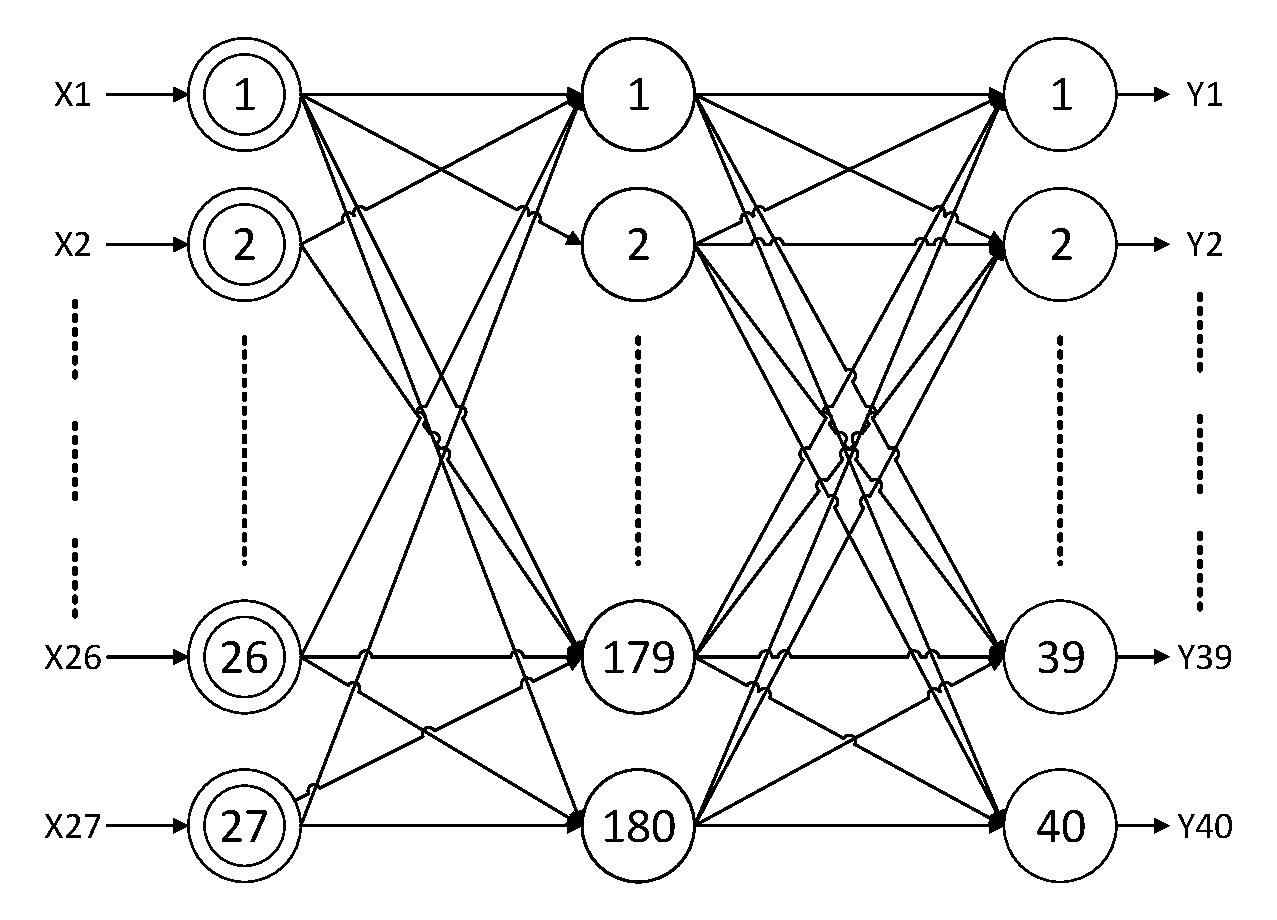
\includegraphics[width=1.0\linewidth]{./img/plots/neural}
     \caption{Design of the Neural Network}
     \label{fig:PerceptronModel}
\end{figure}

\end{document}